\documentclass[AMA,STIX1COL, table]{WileyNJD-v2}
\usepackage{placeins}
\PassOptionsToPackage{table}{xcolor}
\usepackage{pdflscape}
\usepackage{threeparttable}

\articletype{RESEARCH REPORT}%

\raggedbottom

\begin{document}

\title{The harm of SMOTE and other imbalance adjustments: a case study}

\author{Ruben van den Goorbergh}



\authormark{Ruben van den Goorbergh}

\corres{Ruben van den Goorbergh, Julius Center for Health Sciences and Primary Care,University Medical Center Utrecht,Utrecht University, P.O. Box 85500, 3508GA Utrecht, The Netherlands. \email{r.w.vandengoorbergh@uu.nl}}



\abstract[Summary]{In machine learning applications, class imbalance is often adjusted for using data pre-processing methods. I present a case study showing the effect of pre-processing methods on the model performance in low dimensional data. All pre-processing methods yield prediction models that overestimate the risk predictions while not improving the discriminative ability. I advise to apply great caution when using imbalance adjustments if the calibration of the prediction model is of interest.
}

\keywords{Clinical risk prediction models, logistic regression, random forest, gradient boosting machines, XGboost, class imbalance, SMOTE, oversampling, undersampling}


\maketitle



\section{Introduction}
In the field of prediction modelling and machine learning, class imbalance is a well-known phenomenon.\cite{He&Garcia2009} Class imbalance refers to the situation in which the event rate in a data set is not 50\%. \cite{He&Garcia2009} In medical data, the event of interest is often rare or sometimes very rare, which can result in severe class imbalance. The traditional approach for developing dichotomous clinical risk prediction models involves the use of logistic regression models\cite{Christdoulou2019}, which do not necessarily suffer from unevenly distributed classes.\cite{Oommen2011} However, imbalanced data may lead to problems for many other machine learning algorithms because of their accuracy-oriented design, resulting in overlooking the minority class.\cite{Fernandez2018} Therefore, solutions to imbalanced data could be of great interest for clinical prediction modelers, as interest in exploiting complex machine learning models is growing.\cite{Christdoulou2019}

One category of solutions for dealing with imbalanced data is to pre-process the data using resampling techniques, where part of the data in the majority class is discarded (undersampling) or the data of the minority class is duplicated (oversampling). This results in an artificial, more balanced data set. \cite{He&Garcia2009}\cite{Fernandez2018} However, in a medical setting, it is of paramount importance that the prediction model is not only able to accurately distinguish events and non-events, but also able to accurately estimate the risk of event (i.e. the calibration of the model is important). This means that there should be an overall agreement between the observed outcomes and risk estimates.\cite{Steyerberg2009} Combining the notion of calibration with the fact that, in medicine, the diseases and other health outcomes we want to predict often lead to imbalanced data sets, raises the question how adjustments made for class imbalance affect the performance of the models used for making these predictions.

In this research report, I will investigate the performance of two regression-based models (regular- and ridge logistic regression) and two tree-based models (random forest and gradient boosting) for dichotomous risk prediction on imbalanced data. The study focuses on both the discriminative performance and calibration of these models when the imbalance is either adjusted for by one of the following data pre-processing methods: random undersampling (RUS), random oversampling (ROS) or Synthetic Minority Oversampling Technique (SMOTE). \cite{Smote2018}


This report is structured as follows. In the next section, I will describe the used models, class imbalance approaches, performance metrics and data. In section three I present the results of the analysis. In the last section the results are discussed and a simulation study is proposed.  

\section{Methods}

\subsection{Models} \label{models}
\subsubsection{Regression-based models}
In logistic regression the probability $(\pi_i(\mathbf x_i))$ of a positive outcome for person i $(y_i=1)$ is modelled using as set of $R$ predictors $\mathbf x_i$ by estimating regression coefficients $\beta_j$ and intercept $\alpha$. Let $\mathbf{\beta}$ be a column vector containing intercept $\alpha$ and coefficients $\beta_j$, the regression coefficients are estimated maximizing log-likelihood function of the following form

\begin{equation*}
    \label{lr_ll}
    l(\mathbf \beta) = \sum_{i=1}^n \{y_i log(\pi_i(\mathbf{\beta})) + (1 - y_i)log(1 - \pi_i(\mathbf{\beta}))\}
\end{equation*}

In ridge logistic regression\cite{schaefer1984}\cite{lecessie}, the following penalized version of the log likelihood function is used for estimating $\mathbf \beta$, tending to shrink the coefficients towards zero

\begin{equation*}
    \label{ridge_likelihood}
    l(\mathbf \beta) - \lambda \sum_{j = 1}^2 \beta_j^2
\end{equation*}

The hyperparameter $\lambda$ needs to be tuned. In this article it is estimated by minimizing the deviance using 10-fold cross-validation with a grid of 251 possible values for $\lambda$ ranging from 0 (no shrinkage) to 64 (large shrinkage).

\subsubsection{Tree-based models}
Random forest \cite{Breiman2001} and Gradient Boosting Machines both use an ensemble of classification and regression trees (CART) to predict a positive outcome. The Random forest algorithm does this by training each tree on a bootstrapped sample of the development set, using a subset of the predictors to reduce correlation between trees. This process is illustrated with the pseudo-code in algorithm \ref{algRF}. To get to a prediction, the results of all trees are combined by means of a majority vote. The estimated probability is simply the fraction of trees that voted positive given a particular combination of predictor values. For fitting the model the randomForest \cite{randomForest} package was used with default hyperparameters.



Unlike random forest, Gradient Boosting Machines directly predict probabilities using feature vector $\mathbf{x}$. In this process, an initial tree predicts the probabilities. Each next tree then tries to minimize the differences between the predicted probabilities and the outcome of each observation. In the XGboost \cite{xgboost} implementation of gradient boosting, each new tree is fitted by minimizing the loss function

\begin{equation*}
\label{xg_loss}
\mathcal{L}^t = \sum_{i = 1}^n l(y_i, \hat{y}_i^{(t-1)} + f_t(\mathbf x_i)) + \Omega(f_t) \
\end{equation*}

Where $l$ is the differentiable loss function that measures the difference between estimated probability $\hat{y}_i$ and the observed score $y_i$ for each person $i$. We may notice that the predicted score consists of the score predicted in the last iteration $(\hat{y}_i^{(t-1)})$ plus the leaf scores of the tree in the current iteration $(f_t(\mathbf x_i))$. $\Omega(f_t)$ is a regularization term that prevents the model from overfitting and can be defined as 

\begin{equation*}
\label{xg_regularization}
\Omega(f_t) = \gamma T + \frac{1}{2} \lambda \sum_{j = 1}^T \omega_j^2
\end{equation*}

Where $T$ is the number of terminal leaves, $\omega_j$ is the leaf score of leaf $j$ and $\gamma$ and $\lambda$ are tuneable hyper parameters. For this research both hyperparameters $\gamma$ and $\lambda$ were set to 0, omitting the regularization term. 

Other hyperparameters in the XGboost package that were manually tuned were maximum tree depth, learning rate, number of threads and number of rounds. Tuning these hyperparameters did not seem to substantially affect the results. As every new tree tries to explain the difference between the previous prediction and the outcome, the sum of the predictions of all trees results in the final estimated probability given a combination of predictor values.

\FloatBarrier
\begin{algorithm}[hbt!]
\caption{Pseudo-code for Random Forest \cite{Guo2019}} \label{algRF}
\begin{algorithmic}

  \For {i = 1 to c}
    \State Randomly sample training data $D$ with replacement to produce $D_i$
    \State Create root node $N_i$, containing $D_i$
    \State Call BuildTree$(N_i)$
   
  \EndFor
  
\textbf{BuildTree(N)}
 
    \If{$N$ contains instances of only one class}
        \State \textbf{Return}
    \Else
        \State Randomly  select x\% of possible splitting features in N
        \State Select feature F
        \State Create f child nodes of $N, N_1, ..., N_f$, where $F$ has $f$ possible values $(F_1, ..., F_f)$
   
   
   \For {$i = 1$ to $f$} 
     \State Set the contents of $N_i$ to $D_i$, where $D_i$ is all instances in $N$ that match $F_i$
     \State Call BuildTree($N_i$)
   \EndFor
   \EndIf
   
\end{algorithmic}
\end{algorithm}
\FloatBarrier


\subsection{Solutions imbalanced data}
To create a balanced data set, that is, a data set where there are the same number of events as non-events, several approaches have been proposed in the machine learning literature. Three of these approaches are examined in this paper.

In ROS, the size of the minority class is increased by resampling cases from the minority class with replacement until it has the same size as the majority class. This means that the new data set contains duplicate cases for the minority class. In RUS, the size of the majority class is reduced to the size of the minority class by randomly discarding cases from the majority class. 

SMOTE is a form of oversampling where new synthetic cases are created. These synthetic cases are created by operating in the "feature space" instead of the "data space".\cite{Chawla2002} \cite{Smote2018} That is, each synthetic case is created by sampling a random case from the minority class after which its \emph{k} nearest neighbours are determined. In the {\fontfamily{qcr}\selectfont smotefamily} R package I used to implement SMOTE, the nearest neighbours are determined based on the Euclidean distance.\cite{smotefamily}\cite{FNN} Then the differences between the feature vectors of the sampled case and those of its \emph{k} nearest neighbours is taken. These differences are then multiplied by a random number between 0 and 1 and are added to the feature vector of the initial case. This results in \emph{k} synthetic cases that are interpolated from the original minority class cases. By adding these cases to the data set, balance is achieved.
    


\subsection{Data} \label{sec3}
For this study, I used a subset of the data from the International Ovarian Tumor Analysis (IOTA) consortium containing only woman who are not yet in their menopause. \cite{VanCalster2014} The data are derived from 5914 patients between 1999 and 2012. The subset contains data of 3488 patients. A subset of the data was used to achieve a data set with a higher imbalance ratio than the full data set. As outcome variable I used the final diagnoses whether the tumor was benign (n = 2785, 79.8\%) or malignant (n = 703, 20.2\%). The features considered as predictors are: age and diameters of the ovary (ovaryd1 and ovaryd3).



\subsection{Analytic strategy} \label{sec4}
To assess the performance of the different approaches to deal with imbalanced data in combination with the different models, the data was first randomly split up in to a validation and a development set using a 1:4 ratio. Afterwards the development data set was used to create multiple training data sets using random oversampling, random undersampling and SMOTE, resulting in four different data sets; $D_{unadjusted},D_{over}, D_{under}, D_{SMOTE}$.

For every development set $D_i$, the prediction models as described in section \ref{models} were trained with the aim to distinguish between benign and malignant tumors based on the predictors, resulting in 16 (4 x 4) different models. Subsequently all models were assessed on their performance predicting the outcome of the cases contained in the validation set. More information on how the performance evaluation was done can be found in section \ref{sec5}.

\subsection{Performance evaluation} \label{sec5}
To quantify the out of sample performance of the model in terms of discrimination, I considered the c-statistic (area under the ROC curve).\cite{Hanley1982} To asses calibration, I made use of both a visual representation of the calibrative performance of the models in the form of calibration plots and quantitative performance measures in the form of the Estimated Calibration Index (ECI)\cite{Hoorde2015}, calibration slopes and calibration intercepts. \cite{Cox1958} \cite{Miller1991} 

The c-statistic can be interpreted as the probability that a random pair of a positive and a negative case are correctly ranked (i.e. that the positive case has got assigned a higher probability than the negative case). The confidence interval for the c-statistic is estimated using the method as described by Pepe \cite{Pepe2003} using the {\fontfamily{qcr}\selectfont auRoc}\cite{auRoc}R package.

To asses the performance regarding correct classification, I used accuracy, sensitivity and specificity scores. Accuracy can be interpreted as the fraction of correctly classified cases compared to the total number of cases. Sensitivity is the ratio of true positives over the number of positive cases in the data set. Specificity is the ratio of true negatives over the total number of negative cases. All classifications were made using the conventional decision threshold of 0.5. A description of the interpretation of all performance measures can be found in Table \ref{tab1}. 



\FloatBarrier
\begin{center}
\begin{threeparttable}[hbt!]
\renewcommand{\arraystretch}{1.5}

\centering
\caption{Performance measures\label{tab1}}%
\rowcolors{2}{gray!25}{white}
\begin{tabular*}{454}{lc}%
\toprule
\textbf{Performance measure} & \textbf{Interpretation}\\
\midrule
Accuracy $\left(\frac{TP + TN}{TP + FP + TN + FN}\right)$ & Fraction correctly classified cases \\
Sensitivity $\left(\frac{TP}{TP + FN}\right)$ & Fraction correctly classified positive cases over all positive cases \\
Specificity $\left(\frac{TN}{FP + TN}\right)$ & Fraction correctly classified negative cases over all negative cases \\
& c-statistic = 1: perfect discrimination \\
\multirow{-2}{4em}{\cellcolor{gray!25}c-statistic} & \cellcolor{gray!25}c-statistic = 0.5: no discriminative performance \\
\cellcolor{white}& \cellcolor{white} ECI = 0: No difference between observed and predicted probability\\
\multirow{-2}{4em}{ECI} & ECI = 100: maximum difference between observed and predicted probability\\
& Calibration slope < 1: underfitting \\
\multirow{-2}{4em}{\cellcolor{gray!25}Calibration slope} & \cellcolor{gray!25}Calibration slope > 1: overfitting \\
\cellcolor{white}& \cellcolor{white}Calibration intercept = 0: mean calibration is perfect\\
& Calibration intercept > 0: probabilities are systematically too high\\
\multirow{-3}{4em}{\cellcolor{white}Calibration intercept} & \cellcolor{white}Calibration intercept < 0: probabilities are systematically too low\\
\cellcolor{gray!25}Calibration curve & \cellcolor{gray!25}The further the curve from the diagonal, the worse the calibrative performance \\
\bottomrule
\end{tabular*}
\begin{tablenotes}%%[341pt]
\item Abbreviations: TP = True postive, TN = True negative, FP = False positive, FN = False negative, ECI = Estimated Calibration Index
\end{tablenotes}
\end{threeparttable}
\end{center}
\FloatBarrier

\subsection{Software}
All analyses were performed using {\fontfamily{qcr}\selectfont R version 3.6.2}.\cite{R} To fit the regression and machine learning models, I used the following R packages: {\fontfamily{qcr}\selectfont
glmnet} \cite{glmnet}, 
{\fontfamily{qcr}\selectfont randomForest}\cite{randomForest}, 
{\fontfamily{qcr}\selectfont XGboost}\cite{xgboost}. For the random over- and undersampling procedure I used the {\fontfamily{qcr}\selectfont caret}\cite{caret} R package and to implement SMOTE I used the {\fontfamily{qcr}\selectfont smotefamily}\cite{smotefamily} R package.


\section{Results}
For all imbalance adjustment approaches and prediction models, it can be seen from the calibration plots that the predicted probabilities exceeded the observed probabilities over the whole scale (Figure 1). This means that the estimated probabilities tended to be to high compared to the observed probability. This observation was confirmed by the calibration in the large (CIL) statistics in Table \ref{tab2}, which were all >0 for the models trained on the adjusted data sets. 

%%%%%%%%%%%%%%%%%%%%% Add paragraph on slope?
Although the ECI statistic on itself has no straightforward interpretation, it can be used to compare overall performance in terms of calibration. The ECI scores in Table \ref{tab2} showed the same picture of the calibration being affected by data pre-processing, as for all modelling algorithms the lowest ECI was the one for the model that was trained on the data set where the data remained unadjusted for class imbalance. 

	
The c-statistics did not show a noticeable difference over the different models, indicating that the imbalance approaches did not improve the overall discriminative performance of the models. The accuracy tended to be the highest for the models trained on data sets where the imbalance was not adjusted for (Table \ref{tab2}), indicating that the number of correct predictions was the highest using these models. However, differences did occur when looking at the sensitivity and specificity over different scenarios. In the cases where the data was adjusted, the sensitivity and specificity tended to have more similar values, where the in the cases where the data remained unadjusted the minority class was overlooked. For instance the sensitivity of the logistic regression model trained on the unadjusted data had a sensitivity score of no more than 0.15, meaning that only 15\% of the minority class cases in the validation set got detected by the model. 

\FloatBarrier
\begin{figure}[hbt!]
    \centering
    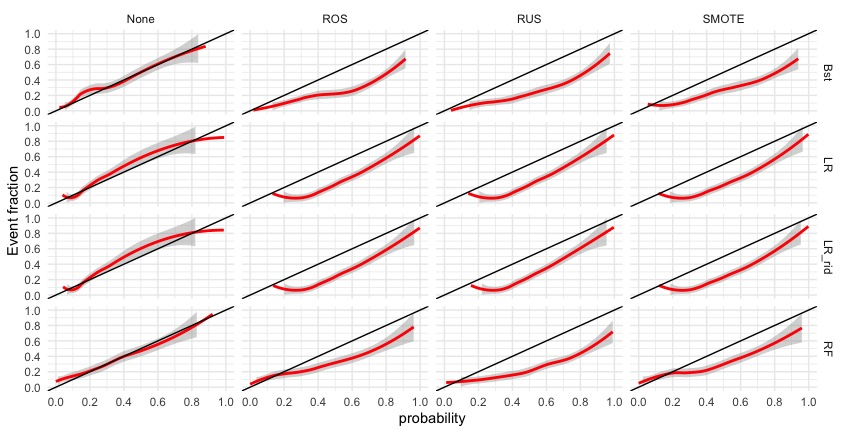
\includegraphics[scale = 0.55]{Rplot03.jpeg}
    \caption{Calibration plots. The red line shows the loess curve fitted on the predicted probabilities. The dark grey area shows the 95\% confidence interval of the loess curve. The black line shows the hypothetical situation of perfect predictions. Abbreviations: LR = Regular Logistic Regression, LR\_rid = Ridge Logistic Regression, RF = Random Forest, Bst = Gradient Boosting Machine, ROS = Random Oversampling, RUS = Random Undersampling, SMOTE = Synthetic Minority Oversampling Technique}
    \label{fig1}
\end{figure}

\FloatBarrier

\begin{landscape}

\begin{threeparttable}

\centering
\caption{Performance of models in combination with data adjustments for handling class imbalance\label{tab2}}%
\begin{tabular}{lllllllll}
  \toprule
 & Adjustment & Accuracy & Sensitivity & Specificity & c-statistic (CI) & CIL (CI) & Calibration slope (CI) & ECI \\ 
  \midrule
&None & 0.81 & 0.15 & 0.98 & 0.76 (0.71 — 0.80) & 0.09 (-0.11 — 0.28) &1.18 (0.93 — 1.45) & 0.16 \\ 
  &ROS & 0.72 & 0.64 & 0.74 & 0.76 (0.71 — 0.80) & -1.28 (-1.48 — -1.09) & 1.13 (0.88 — 1.39) & 5.77 \\ 
  &RUS & 0.72 & 0.64 & 0.74 & 0.76 (0.71 — 0.80) & -1.28 (-1.48 — -1.09) & 1.18 (0.92 — 1.45) & 5.93 \\ 
  \multirow{-2}{4em}{LR}&SMOTE & 0.72 & 0.66 & 0.74 & 0.76 (0.71 — 0.80) & -1.29 (-1.49 — -1.09) & 1.08 (0.85 — 1.33) & 5.77 \\ 
  \midrule
  &None & 0.81 & 0.14 & 0.98 & 0.76 (0.71 — 0.80) & 0.09 (-0.11 — 0.28) & 1.22 (0.96 — 1.50) & 0.19 \\ 
  &ROS & 0.72 & 0.64 & 0.75 & 0.76 (0.71 — 0.80) & -1.28 (-1.48 — -1.08) & 1.14 (0.90 — 1.40) & 5.78 \\ 
  &RUS & 0.72 & 0.64 & 0.74 & 0.76 (0.71 — 0.80) & -1.28 (-1.48 — -1.09) & 1.24 (0.98 — 1.53) & 6.01 \\ 
  \multirow{-2}{4em}{$LR_{rid}$}&SMOTE & 0.72 & 0.66 & 0.74 & 0.76 (0.71 — 0.80) & -1.29 (-1.49 — -1.09) & 1.09 (0.86 — 1.35) & 5.78 \\ 
  \midrule
  &None & 0.80 & 0.23 & 0.95 & 0.73 (0.68 — 0.77) & 0.27 (0.05 — 0.48) & 0.6 (0.46 — 0.74) & 0.27 \\ 
  &ROS & 0.78 & 0.41 & 0.88 & 0.72 (0.67 — 0.76) & -0.48 (-0.69 — -0.27) & 0.57 (0.43 — 0.71) & 1.50 \\ 
  &RUS & 0.70 & 0.64 & 0.71 & 0.73 (0.68 — 0.77) & -1.37 (-1.58 — -1.16) & 0.67 (0.51 — 0.83) & 6.16 \\ 
  \multirow{-2}{4em}{RF}&SMOTE & 0.78 & 0.42 & 0.88 & 0.71 (0.66 — 0.75) & -0.49 (-0.7 — -0.28) & 0.57 (0.43 — 0.71) & 1.59 \\ 
  \midrule
  &None & 0.82 & 0.28 & 0.97 & 0.76 (0.72 — 0.80) & 0.14 (-0.07 — 0.34) & 0.92 (0.74 — 1.12) & 0.15 \\ 
  &ROS & 0.72 & 0.58 & 0.76 & 0.74 (0.69 — 0.78) & -1.22 (-1.43 — -1.02) & 0.77 (0.60 — 0.94) & 4.77 \\ 
  &RUS & 0.69 & 0.64 & 0.71 & 0.73 (0.69 — 0.78) & -1.36 (-1.57 — -1.15) & 0.77 (0.60 — 0.94) & 5.79 \\ 
  \multirow{-2}{4em}{Bst}&SMOTE & 0.74 & 0.59 & 0.78 & 0.74 (0.70 — 0.79) & -1.17 (-1.38 — -0.96) & 0.78 (0.62 — 0.96) & 4.18 \\ 
   \bottomrule
\end{tabular}
\begin{tablenotes}%%[341pt]
\item Abbreviations: LR = Regular Logistic Regression, $LR_{rid}$ = Ridge Logistic Regression, RF = Random Forest, Bst = Gradient Boosting Machine, ROS = Random Oversampling, RUS = Random Undersampling, SMOTE = Synthetic Minority Oversampling Technique, CIL = Calibration in the large, ECI = Estimated Calibration Index, CI = Confidence Interval
\end{tablenotes}
\end{threeparttable}

\end{landscape}

\section{Discussion}

In this report I conducted a case study to examine the effect of data pre-processing methods to adjust for class imbalance on the performance of medical prediction models. I found that data pre-processing methods can seriously affect the calibration and therefore has implications for the development of these models.

The results show that, when adjusting the data for class imbalance, models tend to overestimate probabilities estimated for the individual cases and thus are poorly calibrated. Van Calster et al.\cite{VanCalster2014} describe this as the lack of mean calibration, the most basal type of calibration. Moreover, imbalance solutions did not seem to improve the performance of the models in terms of the c-statistic. The pre-processing methods did show to bring the sensitivity and specificity closer to each other, indicating that these methods do help to increase the model performance in terms of correctly classifying the minority class. However, it can be argued that this could also be done by moving the decision threshold value so that the calibration is not affected. \cite{Collell2018}  

This study has also some limitations. First of all, the absence of weighting as a solution for imbalanced data in this paper can be seen as a limitation, since it is a method that is sometimes used to deal with class imbalance.\cite{Christdoulou2019} Yet, as Maloof points out\cite{Maloof2003}, weighting and oversampling are conceptually closely related and have very similar results. Secondly, as a result of being a case study based on only one data set, it is not possible to generalize findings to a broad set of scenarios that may be encountered in the development of medical prediction models. Another limitation related to this is that the imbalance ratio in the used data set is not as extreme as it can be in medical data sets.\cite{khalilia} To overcome the lack of generalizability, for my master thesis I will build on these results by conducting an elaborate simulation study varying the event fraction and the number of events per variable. 

In conclusion, prediction modelers should be careful when applying class imbalance solutions when calibration of the prediction model is important. The case study illustrates that miscalibration effects of commonly used solution approaches can be strong, future research should elucidate the consequences of these solutions in different scenarios.   


\bibliography{wileyNJD-AMA}


\clearpage




\end{document}






